%%%% main.tex -- IJCAI-27 submission draft (anonymous): Upright kNN
%   build: bash build.sh (pdflatex -> bibtex -> pdflatex x2); numbers and table bodies come from gen/mk_ijcai.py (numbers.tex, tab_*.tex),
%   Figure 1(b) from gen/mk_fig1_en.py; template files ijcai27.sty / named.bst of the official IJCAI-27 kit (unchanged).
\typeout{IJCAI--27 submission: Upright kNN}
\documentclass{article}
\pdfpagewidth=8.5in
\pdfpageheight=11in
\usepackage{ijcai27}
\usepackage{times}
\usepackage{soul}
\usepackage{url}
\usepackage[table]{xcolor}
\usepackage[hidelinks]{hyperref}
\usepackage[utf8]{inputenc}
\usepackage[small]{caption}
\usepackage{graphicx}
\usepackage{amsmath}
\usepackage{amssymb}
\usepackage{amsthm}
\usepackage{booktabs}
\usepackage{algorithm}
\usepackage{algorithmic}
\usepackage[switch]{lineno}
\usepackage{tikz}
\usetikzlibrary{arrows.meta,positioning,calc,fit}
\linenumbers   % comment out in the camera-ready version
\urlstyle{same}
\newtheorem{proposition}{Proposition}
\pdfinfo{
/TemplateVersion (IJCAI.2027.0)
}
\definecolor{firstblue}{RGB}{189,215,238}
\definecolor{navyc}{RGB}{31,58,122}\definecolor{redc}{RGB}{192,57,43}
\newcommand{\veps}{\boldsymbol{\varepsilon}}
\newcommand{\Rot}[1]{\mathbf{R}_{#1}}
\newcommand{\Vf}{\mathbf{V}}\newcommand{\Hf}{\mathbf{H}}
\newcommand{\mG}{\mathcal{G}}
\newcommand{\up}{\mathrm{up}}
\makeatletter\newcommand{\inputrows}[1]{\@@input #1 }\makeatother   % primitive \input inside tabular (a rule may follow)
% written by gen/mk_ijcai.py
\newcommand{\nPairs}{63}
\newcommand{\oursMean}{93.4}
\newcommand{\tunedMean}{92.6}
\newcommand{\ctMean}{87.7}
\newcommand{\rotMean}{84.0}
\newcommand{\cfsMean}{82.4}
\newcommand{\cfsKnnMean}{85.5}
\newcommand{\bestEightName}{MSMA$^{*}$}
\newcommand{\bestEightMean}{80.5}
\newcommand{\bestPriorMean}{85.5}
\newcommand{\priorGap}{7.9}
\newcommand{\priorWinMin}{41}
\newcommand{\priorWinMax}{62}
\newcommand{\priorLossMax}{4}
\newcommand{\nPrior}{11}
\newcommand{\wtlTuned}{30/32/1}
\newcommand{\wtlCfsKnn}{48/15/0}
\newcommand{\wtlRot}{41/18/4}
\newcommand{\nNatPairsMain}{47}
\newcommand{\priorWinMinNat}{35}
\newcommand{\priorWinMaxNat}{47}
\newcommand{\priorLossMaxNat}{2}
\newcommand{\wtlTunedNat}{24/22/1}
\newcommand{\wtlKnnTNat}{28/18/1}
\newcommand{\wtlPoseNat}{29/14/4}
\newcommand{\winKnnTNat}{28}
\newcommand{\lossKnnTNat}{1}
\newcommand{\gainKnnTNat}{0.9}
\newcommand{\knnTCten}{93.7}
\newcommand{\knnTIN}{77.0}
\newcommand{\knnTMean}{92.5}
\newcommand{\nLostNat}{3}
\newcommand{\nNoLossNat}{44}
\newcommand{\nNoLoss}{56}
\newcommand{\nLost}{7}
\newcommand{\vfTunedFourRange}{50--77}
\newcommand{\vfOursAvg}{86.6}
\newcommand{\vfTunedAvg}{72.7}
\newcommand{\vfRotAvg}{94.6}
\newcommand{\vfPoseAvg}{94.7}
\newcommand{\vfCfsKnnAvg}{70.6}
\newcommand{\vfIN}{80.4}
\newcommand{\vfINT}{50.5}
\newcommand{\vfSVHN}{64.5}
\newcommand{\vfSVHNPose}{78.6}
\newcommand{\contentMean}{92.5}
\newcommand{\poseMean}{89.9}
\newcommand{\pChCten}{64.1}
\newcommand{\pChCtenT}{66.6}
\newcommand{\poseChCten}{28.4}
\newcommand{\pCtenCh}{80.3}
\newcommand{\pCtenChT}{77.1}
\newcommand{\poseCtenCh}{86.0}
\newcommand{\contentCtenCh}{77.4}
\newcommand{\pInInat}{71.9}
\newcommand{\pInInatNLL}{84.4}
\newcommand{\oursCten}{95.4}
\newcommand{\tunedCten}{93.7}
\newcommand{\oursIN}{79.6}
\newcommand{\tunedIN}{77.0}
\newcommand{\FPRours}{26.5}
\newcommand{\FPRbest}{29.8}
\newcommand{\FPRbestPriorName}{Rotation pred.}
\newcommand{\FPRbestPrior}{43.5}
\newcommand{\cpuOurs}{0.18}
\newcommand{\cpuNll}{58}
\newcommand{\cpuDiffPath}{2.0}
\newcommand{\cpuCfs}{0.21}
\newcommand{\cpuEigen}{40}
\newcommand{\cpuRot}{0.03}
\newcommand{\cpuRatioNll}{320}
\newcommand{\cpuRatioDiffPath}{11}
\newcommand{\dimRange}{14--25}
\newcommand{\headAccRange}{77--100}
\newcommand{\leakAccIN}{91.6}
\newcommand{\cleanAccIN}{77.3}
\newcommand{\devOurs}{93.3}
\newcommand{\devTuned}{92.5}
\newcommand{\abNatA}{93.4}
\newcommand{\abVfA}{86.4}
\newcommand{\abSelA}{93.3}
\newcommand{\abNatB}{92.4}
\newcommand{\abVfB}{72.7}
\newcommand{\abSelB}{93.0}
\newcommand{\abNatC}{89.8}
\newcommand{\abVfC}{94.7}
\newcommand{\abSelC}{87.6}
\newcommand{\abNatD}{93.3}
\newcommand{\abVfD}{87.7}
\newcommand{\abSelD}{93.2}
\newcommand{\abNatE}{93.1}
\newcommand{\abVfE}{92.3}
\newcommand{\abSelE}{92.5}
\newcommand{\abNatF}{92.6}
\newcommand{\abVfF}{86.5}
\newcommand{\abSelF}{92.9}
\newcommand{\abNatG}{92.9}
\newcommand{\abVfG}{78.8}
\newcommand{\abSelG}{93.1}
\newcommand{\abNatH}{92.9}
\newcommand{\abVfH}{88.1}
\newcommand{\abSelH}{93.2}
\newcommand{\abInVfLeak}{71.9}
\newcommand{\abInVfNoT}{82.6}
\newcommand{\abCtenOurs}{95.9}
\newcommand{\abCtenOrbit}{91.8}
\newcommand{\inNear}{70.2}
\newcommand{\inFar}{79.0}
\newcommand{\inNearPrior}{60.7}
\newcommand{\inFarPrior}{75.0}
\newcommand{\inSSB}{68.6}
\newcommand{\inNINCO}{71.9}
\newcommand{\inInat}{70.1}
\newcommand{\inTex}{93.2}
\newcommand{\inOIO}{73.9}
\newcommand{\inInatNLL}{83.8}
\newcommand{\inInatTT}{74.0}
\newcommand{\inVtwo}{52.4}
\newcommand{\inC}{92.3}
\newcommand{\inR}{77.9}
\newcommand{\inFSnear}{53.9}
\newcommand{\inFSfar}{63.3}
\newcommand{\inFSnearNLL}{56.5}
\newcommand{\inFSfarNLL}{69.3}
\newcommand{\inCNLL}{43.3}
\newcommand{\inRNLL}{31.3}
\newcommand{\inNearFPR}{83.9}
\newcommand{\inFarFPR}{74.4}
\newcommand{\inNearKnnT}{69.5}
\newcommand{\inFarKnnT}{76.4}
\newcommand{\inNearPose}{63.5}
\newcommand{\inFarPose}{77.4}
\newcommand{\inNearFull}{70.6}
\newcommand{\inFarFull}{79.3}
\newcommand{\inCsevOne}{88.4}
\newcommand{\inCsevFive}{94.5}
\newcommand{\inPriorWinMin}{4}
\newcommand{\inPriorLossMax}{1}
\newcommand{\inLossRows}{NLL, TT}
\newcommand{\inNFull}{42{,}000}
\newcommand{\fuRZ}{91.2}
\newcommand{\fuRZvf}{92.4}
\newcommand{\fuRZwtl}{30/17/0}
\newcommand{\fuRF}{91.2}
\newcommand{\fuRFvf}{92.9}
\newcommand{\fuRFwtl}{19/26/2}
\newcommand{\fuOZ}{93.1}
\newcommand{\fuOZvf}{92.4}
\newcommand{\fuOZwtl}{23/17/7}
\newcommand{\fuOF}{93.1}
\newcommand{\fuOFvf}{92.5}
\newcommand{\fuOFwtl}{13/26/8}
\newcommand{\fuDO}{92.0}
\newcommand{\fuDOvf}{94.2}
\newcommand{\fuDOwtl}{24/20/3}
\newcommand{\nNatPairs}{47}
\newcommand{\hNINCO}{80.6}
\newcommand{\hFar}{72.2}
\newcommand{\hVf}{78.5}
\newcommand{\hInat}{84.1}
\newcommand{\hTex}{78.5}
\newcommand{\hOIO}{54.0}
\newcommand{\hNINCOKnnT}{81.4}
\newcommand{\hVfKnnT}{50.6}
\newcommand{\hVfPose}{92.6}
\newcommand{\hNcom}{500}
\newcommand{\hSSB}{93.7}
\newcommand{\hSSBCfs}{85.4}
\newcommand{\hSSBKnnB}{78.5}
\newcommand{\hNINCOPrior}{65.9}
\newcommand{\hNINCOPriorName}{CFS (kNN head)}
\newcommand{\hFarPrior}{74.1}
\newcommand{\hFarPriorName}{CFS (diag.)}
\newcommand{\hFarVerdictCfs}{tie}
\newcommand{\hTexCfs}{88.5}
\newcommand{\hOIOCfs}{76.5}
\newcommand{\hTexMsma}{88.2}
\newcommand{\hOIOMsma}{79.5}
\newcommand{\hVfOtherMax}{50.8}
\newcommand{\hVtwo}{56.9}
\newcommand{\hC}{92.9}
\newcommand{\hR}{77.9}
\newcommand{\hSeeds}{3}
\newcommand{\hCfsSeeds}{3}
\newcommand{\hTempRange}{0.88--0.89}
\newcommand{\eOurs}{99.8}
\newcommand{\eKnnT}{99.8}
\newcommand{\ePose}{96.1}
\newcommand{\eKnnB}{99.7}
\newcommand{\eVf}{64.0}
\newcommand{\eRot}{75.8}
\newcommand{\eVfKnnT}{54.2}
\newcommand{\eRotKnnT}{55.1}
\newcommand{\eVfPose}{75.6}
\newcommand{\eRotPose}{91.1}
\newcommand{\eWtlKnnT}{8/1/1}
\newcommand{\eWtlKnnB}{8/1/1}
\newcommand{\eMeanVerdictKnnT}{tie}
\newcommand{\eAcc}{72--74}
\newcommand{\eT}{0.91--0.94}


\title{Upright kNN: Completing Nearest-Neighbour Density on Diffusion Features\\with the Missing Orientation Factor for Out-of-Distribution Detection}
\author{Anonymous Submission}

\begin{document}
\maketitle
\begin{figure*}[t]\centering
\makebox[\textwidth][l]{\small (a) Overview}\\[0.3mm]
\resizebox{\textwidth}{!}{% fig_method.tex -- Figure 1(a) of the IJCAI draft: overview of Upright kNN (TikZ, outlines only); test time on top, the ID-only training of the MLP below
\begin{tikzpicture}[font=\scriptsize, >={Stealth[length=1.5mm]},
  box/.style={draw, rounded corners=1.5pt, align=center, inner sep=2.2pt, minimum height=7.5mm},
  term/.style={box, line width=0.9pt},
  lab/.style={align=center, font=\tiny, inner sep=1pt}]
\node[inner sep=0] (x) {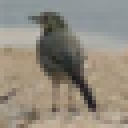
\includegraphics[width=0.95cm]{figs/ex_id.png}};
\node[below=0.4mm of x, inner sep=0] {image $\mathbf{x}$};
\node[box, right=7mm of x] (den) {frozen denoiser\\(one pass)};
\node[box, right=3mm of den] (feat) {last decoder block\\at 3 resolutions};
\coordinate (br) at ($(feat.east)+(2mm,0)$);
\node[box, anchor=west] (knn) at ($(br)+(15mm,8mm)$) {kNN: $R$-th similarity\\$c_R(\mathbf{x})$ to the bank};
\node[box, anchor=west, minimum width=25mm] (mlp) at ($(br)+(15mm,-8mm)$) {small MLP $q_\phi$};
\node[term, draw=navyc, right=2.5mm of knn] (t1) {$-d\log r_R(\mathbf{x})$\\{\tiny estimates $\log\bar p(\mathbf{x})$}};
\node[term, draw=redc, right=2.5mm of mlp] (t2) {$\log q_\phi(\Rot{0}\mid\mathbf{x})$\\{\tiny estimates $\log P(\mathrm{up}\mid\mathbf{x})$}};
\coordinate (mid) at ($(t1.east)!0.5!(t2.east)+(4mm,0)$);
\node[draw, circle, inner sep=0.8pt] (plus) at (mid) {$+$};
\node[right=1mm of plus, align=center] (s) {$s(\mathbf{x})$\\{\tiny ID score}};
\draw[->] (x) -- node[above, lab] {$+\sigma_1\veps$} (den);
\draw[->] (den) -- (feat);
\draw (feat.east) -- (br);
\draw[->] (br) |- node[pos=0.72, above, lab] {channel mean, std} (knn.west);
\draw[->] (br) |- node[pos=0.72, below, lab] {+ 2$\times$2 quadrants} (mlp.west);
\draw[->] (knn) -- (t1); \draw[->] (mlp) -- (t2);
\draw[->] (t1.east) -| (plus.north); \draw[->] (t2.east) -| (plus.south); \draw[->] (plus) -- (s);
\node[anchor=north east, align=left, inner sep=1pt] (trt) at ($(t2.south east)+(0,-5mm)$) {offline, ID images only ($\approx$10\,s): predict the angle $r$ of\\rotated bank images (\textbf{the noise is not rotated})};
\node[inner sep=0, left=2mm of trt] (r3) {\rotatebox{270}{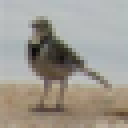
\includegraphics[width=0.42cm]{figs/ex_id_nn0.png}}};
\node[inner sep=0, left=0.7mm of r3] (r2) {\rotatebox{180}{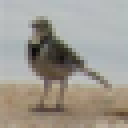
\includegraphics[width=0.42cm]{figs/ex_id_nn0.png}}};
\node[inner sep=0, left=0.7mm of r2] (r1) {\rotatebox{90}{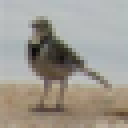
\includegraphics[width=0.42cm]{figs/ex_id_nn0.png}}};
\node[inner sep=0, left=0.7mm of r1] (r0) {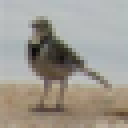
\includegraphics[width=0.42cm]{figs/ex_id_nn0.png}};
\node[draw, dashed, rounded corners=1.5pt, fit=(r0)(r3)(trt), inner sep=1.2mm] (tr) {};
\draw[->, dashed] (tr.north -| mlp.south) -- (mlp.south);
\end{tikzpicture}
}\\[2mm]
\makebox[\textwidth][l]{\small (b) Three examples (CIFAR-10 as ID; development images chosen by a fixed rule)}\\[0.6mm]
\resizebox{0.86\textwidth}{!}{% written by gen/mk_fig1_en.py (Figure 1(b))
\begin{tikzpicture}[font=\scriptsize]
\node[anchor=south] at (1.75,0.62) {input $\mathbf{x}$};
\node[anchor=south] at (3.85,0.62) {nearest bank images};
\node[anchor=south, align=center] at (6.6,0.62) {kNN term\\[-1pt]{\tiny(percentile among ID)}};
\node[anchor=south, align=center] at (9.34,0.62) {posterior $q_\phi(\Rot{r}\mid\mathbf{x})$\\[-1pt]{\tiny($r$ in degrees)}};
\node[anchor=south, align=center] at (12.0,0.62) {score $s(\mathbf{x})$\\[-1pt]{\tiny(percentile among ID)}};
\node[anchor=south] at (13.45,0.62) {decision};
\node at (0.0,0.0) {ID};
\node[inner sep=0] at (1.75,0.0) {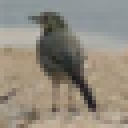
\includegraphics[width=1.0cm]{figs/ex_id.png}};
\node[inner sep=0] at (3.0500000000000003,0.0) {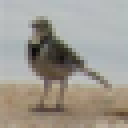
\includegraphics[width=0.78cm]{figs/ex_id_nn0.png}};
\node[inner sep=0] at (3.9000000000000004,0.0) {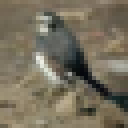
\includegraphics[width=0.78cm]{figs/ex_id_nn1.png}};
\node[inner sep=0] at (4.75,0.0) {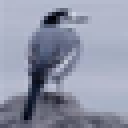
\includegraphics[width=0.78cm]{figs/ex_id_nn2.png}};
\draw[line width=0.4pt] (5.75,-0.11) rectangle (7.45,0.11);
\fill[navyc] (5.75,-0.11) rectangle (6.530,0.11);
\node[anchor=north] at (6.6,-0.12) {\tiny 46\%};
\draw[line width=0.4pt] (11.15,-0.11) rectangle (12.85,0.11);
\fill[black] (11.15,-0.11) rectangle (12.000,0.11);
\node[anchor=north] at (12.0,-0.12) {\tiny 50\%};
\fill[redc] (8.55,-0.42) rectangle (8.75,0.420);
\node[anchor=north, inner sep=1pt] at (8.65,-0.42) {\tiny 0};
\fill[black!45] (9.010000000000002,-0.42) rectangle (9.21,-0.420);
\node[anchor=north, inner sep=1pt] at (9.110000000000001,-0.42) {\tiny 90};
\fill[black!45] (9.47,-0.42) rectangle (9.67,-0.420);
\node[anchor=north, inner sep=1pt] at (9.57,-0.42) {\tiny 180};
\fill[black!45] (9.930000000000001,-0.42) rectangle (10.13,-0.420);
\node[anchor=north, inner sep=1pt] at (10.030000000000001,-0.42) {\tiny 270};
\draw[line width=0.3pt] (8.47,-0.42) -- (10.21,-0.42);
\node[text=navyc] at (13.45,0.0) {\textbf{ID}};
\node[align=center] at (0.0,-1.32) {ID, upside\\down};
\node[inner sep=0] at (1.75,-1.32) {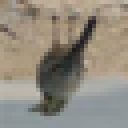
\includegraphics[width=1.0cm]{figs/ex_vflip.png}};
\node[inner sep=0] at (3.0500000000000003,-1.32) {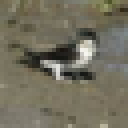
\includegraphics[width=0.78cm]{figs/ex_vflip_nn0.png}};
\node[inner sep=0] at (3.9000000000000004,-1.32) {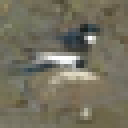
\includegraphics[width=0.78cm]{figs/ex_vflip_nn1.png}};
\node[inner sep=0] at (4.75,-1.32) {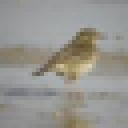
\includegraphics[width=0.78cm]{figs/ex_vflip_nn2.png}};
\draw[line width=0.4pt] (5.75,-1.4300000000000002) rectangle (7.45,-1.21);
\fill[navyc] (5.75,-1.4300000000000002) rectangle (6.105,-1.21);
\node[anchor=north] at (6.6,-1.44) {\tiny 21\%};
\draw[line width=0.4pt] (11.15,-1.4300000000000002) rectangle (12.85,-1.21);
\fill[black] (11.15,-1.4300000000000002) rectangle (11.152,-1.21);
\node[anchor=north] at (12.0,-1.44) {\tiny 0.1\%};
\fill[redc] (8.55,-1.74) rectangle (8.75,-1.740);
\node[anchor=north, inner sep=1pt] at (8.65,-1.74) {\tiny 0};
\fill[black!45] (9.010000000000002,-1.74) rectangle (9.21,-1.740);
\node[anchor=north, inner sep=1pt] at (9.110000000000001,-1.74) {\tiny 90};
\fill[black!45] (9.47,-1.74) rectangle (9.67,-0.900);
\node[anchor=north, inner sep=1pt] at (9.57,-1.74) {\tiny 180};
\fill[black!45] (9.930000000000001,-1.74) rectangle (10.13,-1.740);
\node[anchor=north, inner sep=1pt] at (10.030000000000001,-1.74) {\tiny 270};
\draw[line width=0.3pt] (8.47,-1.74) -- (10.21,-1.74);
\node[text=redc] at (13.45,-1.32) {\textbf{OOD}};
\node[align=center] at (0.0,-2.64) {OOD (Tiny-\\ImageNet)};
\node[inner sep=0] at (1.75,-2.64) {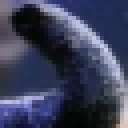
\includegraphics[width=1.0cm]{figs/ex_ood.png}};
\node[inner sep=0] at (3.0500000000000003,-2.64) {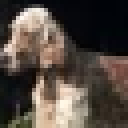
\includegraphics[width=0.78cm]{figs/ex_ood_nn0.png}};
\node[inner sep=0] at (3.9000000000000004,-2.64) {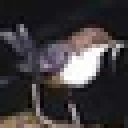
\includegraphics[width=0.78cm]{figs/ex_ood_nn1.png}};
\node[inner sep=0] at (4.75,-2.64) {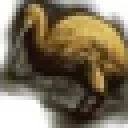
\includegraphics[width=0.78cm]{figs/ex_ood_nn2.png}};
\draw[line width=0.4pt] (5.75,-2.75) rectangle (7.45,-2.5300000000000002);
\fill[navyc] (5.75,-2.75) rectangle (5.769,-2.5300000000000002);
\node[anchor=north] at (6.6,-2.7600000000000002) {\tiny 1.1\%};
\draw[line width=0.4pt] (11.15,-2.75) rectangle (12.85,-2.5300000000000002);
\fill[black] (11.15,-2.75) rectangle (11.169,-2.5300000000000002);
\node[anchor=north] at (12.0,-2.7600000000000002) {\tiny 1.1\%};
\fill[redc] (8.55,-3.06) rectangle (8.75,-2.815);
\node[anchor=north, inner sep=1pt] at (8.65,-3.06) {\tiny 0};
\fill[black!45] (9.010000000000002,-3.06) rectangle (9.21,-3.048);
\node[anchor=north, inner sep=1pt] at (9.110000000000001,-3.06) {\tiny 90};
\fill[black!45] (9.47,-3.06) rectangle (9.67,-2.965);
\node[anchor=north, inner sep=1pt] at (9.57,-3.06) {\tiny 180};
\fill[black!45] (9.930000000000001,-3.06) rectangle (10.13,-2.572);
\node[anchor=north, inner sep=1pt] at (10.030000000000001,-3.06) {\tiny 270};
\draw[line width=0.3pt] (8.47,-3.06) -- (10.21,-3.06);
\node[text=redc] at (13.45,-2.64) {\textbf{OOD}};
\end{tikzpicture}
}
\caption{Upright kNN. (a) At test time, one denoiser pass gives the features of both terms of the score, Eq.~(\ref{eq:score}). (b) From top: the ID image with the median score, the same image upside down, and the Tiny-ImageNet image with the median score of its set. Percentile: fraction of ID images with a lower value; decision: threshold that keeps 95\% of ID images. The flipped image still has a bird as its nearest bank image and its kNN term stays at the 21st percentile, but its orientation posterior moves to $180^\circ$ and its score drops to the 0.1st percentile.}
\label{fig:method}
\end{figure*}

\begin{abstract}
Diffusion models are attractive for unsupervised out-of-distribution (OOD) detection, but their likelihoods are fooled by image complexity and their score statistics cost tens to hundreds of network evaluations per image. A single denoiser pass already gives strong features: a $k$-nearest-neighbour (kNN) rule on channel statistics of decoder activations beats such statistics, yet these features barely encode which way is up, so an upside-down in-distribution image still looks in-distribution. We show that the log-density of an image equals, exactly, the log of its rotation-averaged density plus the log-posterior that the image is upright. Upright kNN estimates the first term with a kNN density on diffusion features and the second with a small MLP trained on rotated in-distribution images in the same feature space, and adds them with weights fixed by the decomposition. Under a protocol frozen before a single evaluation on held-out images (six in-distribution datasets, \nPairs{} pairs, \nPrior{} prior methods), Upright kNN reaches \oursMean\% mean AUROC against \bestPriorMean\% for the best prior method, with one network evaluation per image. On the OpenOOD v1.5 ImageNet-1K benchmark it raises near-/far-OOD AUROC from \inNearPrior/\inFarPrior\% to \inNear/\inFar\% at 64$\times$64; at 256$\times$256, with a different diffusion model and no retuning, it is best on near-OOD NINCO and on upside-down images and ties the best prior method on far-OOD. Naive fusions of kNN with a rotation classifier fall short of it.
\end{abstract}

\section{Introduction}
\label{sec:intro}
A generative model of the training data offers a label-free test for inputs that do not come from the training distribution (out-of-distribution, OOD): such inputs should have low likelihood. Deep generative models, however, often assign higher likelihood to OOD images than to in-distribution (ID) ones~\cite{nalisnick2019deep}, largely because likelihood tracks image complexity~\cite{serra2020input}. Diffusion models~\cite{ho2020ddpm,song2021score} inherit the problem. Detectors built on their score fields, sampling paths or posterior statistics~\cite{mahmood2021msma,heng2024diffpath,alexis2026gepc,shoushtari2026eigenscore} need 10 to 256 network evaluations per image and remain unstable across ID datasets: in our evaluation, the best of eight such detectors averages \bestEightMean\% AUROC over six ID datasets (Table~\ref{tab:main}).

A single denoiser pass is a cheaper and stronger source of evidence. Intermediate activations of a diffusion denoiser are good image representations~\cite{baranchuk2022label,xiang2023ddae}, and CFS~\cite{rouzoumka2026cfs} showed that channel statistics of a few blocks, scored against ID data, beat likelihood- and statistic-based detectors. The kNN rule of \citeauthor{sun2022knn}~\shortcite{sun2022knn} applied to such features is stronger still (\tunedMean\% with a tuned configuration). These features have a blind spot, though: they barely encode which way is up. The tuned kNN separates vertically flipped ID images---same content, wrong orientation---from the originals with only \vfTunedFourRange\% AUROC on four of the six ID datasets. For natural images, being upright is part of what makes an image typical, i.e.\ part of the density $p(\mathbf{x})$.

We make this intuition exact. Let $\bar p$ be the density averaged over the four rotations by multiples of $90^\circ$. Under the mixture of rotated ID images, the posterior probability that $\mathbf{x}$ is upright is $P(\up\mid\mathbf{x})=p(\mathbf{x})/\{4\bar p(\mathbf{x})\}$, so that $\log p=\log\bar p+\log P(\up\mid\cdot)+\log 4$ holds for every image (Proposition~\ref{prop:decomp}). Channel statistics hardly change under rotation, so a kNN density on them mainly estimates the first, orientation-free term; the second term is what is missing. \textbf{Upright kNN} estimates it with a small MLP that is trained, on the features of the same single pass, to predict the rotation of rotated ID images, and it adds the two log-terms with weights fixed by the decomposition (Figure~\ref{fig:method}).

We evaluate under a protocol designed against selection bias: every configuration choice was made on separate selection data, the protocol was frozen, and the final images were evaluated once. Over six ID datasets with public diffusion models (\nPairs{} ID--OOD pairs), Upright kNN reaches \oursMean\% mean AUROC, \priorGap{} points above the best of \nPrior{} prior methods, and it wins \priorWinMin--\priorWinMax{} of the \nPairs{} pairs against each of them at the cost of one network evaluation per image. On ImageNet-1K it improves near- and far-OOD AUROC over the best prior method at 64$\times$64, and at 256$\times$256, with another diffusion model, it is best on near-OOD NINCO and the only method that detects upside-down images. Our contributions are:
\begin{itemize}
\item An exact orientation decomposition of the log-density and Upright kNN, a single-pass, label-free detector that restores the missing orientation factor to a nearest-neighbour density on diffusion features without tuned weights (Section~\ref{sec:method}).
\item A frozen-protocol evaluation on six ID datasets against \nPrior{} prior methods, and on OpenOOD v1.5 ImageNet-1K with near-, far-, covariate-shift and full-spectrum metrics at 64$\times$64 and, with a different diffusion model, at 256$\times$256 (Sections~\ref{sec:setup}--\ref{sec:results}).
\item An analysis of what the orientation factor adds: naive fusions of kNN with a rotation classifier fall short, the exchange rate fixed by the decomposition matters, upside-down images are caught by the second term alone (Proposition~\ref{prop:mirror}), and a label-free mirror test locates orientation information inside the network (Section~\ref{sec:analysis}).
\end{itemize}


\section{Related Work}
\label{sec:related}
\textbf{Likelihoods and score statistics.}
Responses to the likelihood paradox~\cite{nalisnick2019deep} include likelihood ratios~\cite{ren2019lr}, typicality tests~\cite{nalisnick2019typ}, complexity corrections~\cite{serra2020input} and local intrinsic dimension~\cite{kamkari2024geometric}. Diffusion-specific detectors use multiscale score norms (MSMA)~\cite{mahmood2021msma}, reconstruction or inpainting errors~\cite{graham2023ddpmood,liu2023lmd}, statistics of the sampling path (DiffPath)~\cite{heng2024diffpath}, consistency of the posterior mean under transformations (GEPC)~\cite{alexis2026gepc} and eigenvalues of the posterior covariance (EigenScore)~\cite{shoushtari2026eigenscore}. Most need 10 to hundreds of network evaluations per image.

\textbf{Feature-based detection.}
With supervised classifiers, Mahalanobis~\cite{lee2018maha} and deep kNN~\cite{sun2022knn} scores on penultimate features are strong baselines~\cite{yang2024survey,zhang2023openood}. Diffusion denoisers provide features without labels~\cite{baranchuk2022label,xiang2023ddae,tang2023dift}; CFS~\cite{rouzoumka2026cfs} pools channel statistics of one encoder and one decoder block at a single noise level and scores them with a diagonal Gaussian (or, in its appendix, a kNN head). Our kNN term uses the same kind of features; what we add is the orientation factor that the density decomposition shows to be missing.

\textbf{Predicting transformations.}
Classifiers that predict rotations or other geometric transformations of ID images~\cite{gidaris2018rotnet} are used as anomaly scores~\cite{golan2018geometric,hendrycks2019ss}, and contrastive methods such as CSI~\cite{tack2020csi} and SSD~\cite{sehwag2021ssd} learn representations on ID data for the same purpose. These methods train a network from scratch and use the rotation cue as a stand-alone score or as a representation. We train only a small head on frozen diffusion features and use its output as one factor of a density; Section~\ref{sec:fusion} shows that combining kNN with a rotation classifier is not a substitute.

\section{Method}
\label{sec:method}
\textbf{Setting.} We are given ID training images and a diffusion model trained on them; we use its denoiser $D(\mathbf{y};\sigma)$, no labels and no OOD data. A detector assigns a score $s(\mathbf{x})$ that is higher for ID-like images.

\subsection{An Exact Orientation Decomposition}
\label{sec:decomp}
Let $\mG=\{\Rot{0},\Rot{90},\Rot{180},\Rot{270}\}$ be the rotations of the image plane by multiples of $90^\circ$ and define the rotation-averaged density
\begin{equation}
\bar p(\mathbf{x})=\frac{1}{4}\sum_{\mathbf{G}\in\mG}p(\mathbf{G}\mathbf{x}).
\label{eq:pbar}
\end{equation}
Consider the mixture obtained by rotating ID images by an angle drawn uniformly from $\mG$. Rotations permute pixels, so they preserve volume, and $\mG$ is closed under inversion; hence the mixture has density $\frac{1}{4}\sum_{\mathbf{G}}p(\mathbf{G}^{-1}\mathbf{x})=\bar p(\mathbf{x})$, and by Bayes' rule the posterior probability that $\mathbf{x}$ was not rotated is
\begin{equation}
P(\up\mid\mathbf{x})=\frac{p(\mathbf{x})}{4\,\bar p(\mathbf{x})}.
\label{eq:post}
\end{equation}
\begin{proposition}
\label{prop:decomp}
For every image $\mathbf{x}$ with $p(\mathbf{x})>0$,
\begin{equation}
\log p(\mathbf{x})=\log\bar p(\mathbf{x})+\log P(\up\mid\mathbf{x})+\log 4.
\label{eq:decomp}
\end{equation}
\end{proposition}
The identity follows from Eq.~(\ref{eq:post}) by taking logarithms; it is exact and involves no approximation. The first term is a \emph{content} density that does not depend on orientation, since $\bar p(\mathbf{G}\mathbf{x})=\bar p(\mathbf{x})$ for every $\mathbf{G}\in\mG$; the second states how plausible the present orientation is, given the content. A detector that sees only rotation-invariant evidence can at best estimate the first term.

\subsection{The Content Term: a kNN Density on Diffusion Features}
\label{sec:knn}
We add noise $\sigma_1\veps$ to $\mathbf{x}$, with $\sigma_1$ the smallest noise level of the model (0.01 for all models here) and one noise image $\veps$ shared by all images, and pass $\mathbf{x}+\sigma_1\veps$ through the denoiser once. From the last decoder block at full, half and quarter resolution we take the channel-wise spatial mean and standard deviation and normalise each block's vector to unit length. The same features are computed for a bank of ID training images $\mathbf{b}_1,\dots,\mathbf{b}_N$. Let $c_R(\mathbf{x})$ be the $R$-th largest similarity between $\mathbf{x}$ and the bank images (cosine similarity averaged over the three blocks) and $r_R(\mathbf{x})=\sqrt{2\{1-c_R(\mathbf{x})\}}$ the corresponding chordal distance. The kNN density estimate~\cite{loftsgaarden1965knn} in a space of dimension $d$ is proportional to $r_R(\mathbf{x})^{-d}$, so
\begin{equation}
\log\hat{\bar p}(\mathbf{x})=-d\log r_R(\mathbf{x})+\mathrm{const}.
\label{eq:knn}
\end{equation}
We set $d$ to the maximum-likelihood intrinsic dimension~\cite{levina2004mle} of the bank features (20 neighbours; $d=\dimRange$ across our ID datasets). Channel statistics are nearly invariant to rotation, so Eq.~(\ref{eq:knn}) estimates mainly the content term $\log\bar p$; Section~\ref{sec:analysis} measures how much orientation information it still carries. On its own, Eq.~(\ref{eq:knn}) ranks images exactly as the kNN rule with similarity $c_R$ does.

\subsection{The Orientation Term: an Upright Posterior}
\label{sec:pose}
We estimate the second term with a small MLP $q_\phi(\Rot{r}\mid\mathbf{x})$ (one hidden layer of 512 units, four outputs) on features of the same pass: the channel means and standard deviations of the three blocks over the whole image and over each cell of a $2\times2$ grid, standardised on the bank. The grid statistics keep a coarse layout and thus an orientation cue. We hold out 5{,}000 bank images, rotate the remaining ones by each $\Rot{r}\in\mG$, and minimise the cross-entropy of predicting $r$. Because the four angles are equally likely, the minimiser is the posterior of the rotation mixture given the features; it equals Eq.~(\ref{eq:post}) when the features keep the orientation information of the image.

Two details matter. First, the \emph{noise is not rotated}: the inputs are $\Rot{r}\mathbf{b}_i+\sigma_1\veps$. Since $\veps$ is shared, rotating it with the image would let the MLP read the angle from the noise pattern instead of the content; on ImageNet-64 this raises the held-out accuracy from \cleanAccIN\% to \leakAccIN\% but lowers the AUROC on upside-down ID images from \abInVfNoT\% to \abInVfLeak\% (development images, before calibration). Second, we calibrate the posterior with a temperature $T$ that minimises the negative log-likelihood on the held-out bank images~\cite{guo2017calibration}. The head inputs and architecture were chosen by held-out rotation accuracy and likelihood only; the held-out accuracy is \headAccRange\% across ID datasets.

\subsection{The Score}
\label{sec:score}
Replacing both terms of Eq.~(\ref{eq:decomp}) by their estimates gives
\begin{equation}
s(\mathbf{x})=-d\log r_R(\mathbf{x})+\log q_\phi(\Rot{0}\mid\mathbf{x}),
\label{eq:score}
\end{equation}
where constants are dropped because they do not affect rankings. No weight is tuned: the exchange rate between the terms is set by the intrinsic dimension $d$. Since the two terms are estimated on different summaries of the features and the kNN density lives in feature space, Eq.~(\ref{eq:score}) is a plug-in combination guided by Eq.~(\ref{eq:decomp}), not an unbiased estimate of $\log p$. At test time it costs one denoiser pass, inner products with the bank and a 2-ms head on a CPU; offline, it needs one pass over the four rotations of the bank and about 10\,s of MLP training.

\section{Experimental Setup}
\label{sec:setup}
\textbf{ID datasets and models.} We use CIFAR-10~\cite{krizhevsky2009cifar} (EDM~\cite{karras2022edm}), SVHN~\cite{netzer2011svhn} (the VP-SDE of~\citeauthor{kamkari2024geometric}~\shortcite{kamkari2024geometric}), CelebA~\cite{liu2015celeba} (iDDPM~\cite{nichol2021improved}), CIFAR-100 (the EDM-preconditioned DDPM++ of~\citeauthor{chen2024robust}~\shortcite{chen2024robust}), ImageNet-64~\cite{chrabaszcz2017imagenet64} (EDM2-XS, unconditional~\cite{karras2024edm2}) and FashionMNIST~\cite{xiao2017fmnist} (a U-Net we trained). All other weights are public and used unchanged. All images are 32$\times$32 except ImageNet-64.

\textbf{OOD sets.} Each ID dataset is paired with natural OOD datasets (9, 9, 9, 9, 7 and 4 sets; e.g.\ SSB-hard, NINCO, iNaturalist, Textures, OpenImage-O, Places365 and CelebA for ImageNet-64, and greyscale digit and character sets for FashionMNIST), with its own images flipped upside down, and with uniform-noise and constant images (except ImageNet-64): \nPairs{} ID--OOD pairs in total.

\textbf{Protocol.} Images are split into three disjoint parts: (i) selection data (ID development images and 6--11 OOD datasets per ID dataset that are never used for evaluation), (ii) development evaluation images (1{,}000 per set) and (iii) final evaluation images (500 per set). All configuration choices of Upright kNN ($R$ and the blocks of the kNN term) were made on (i), the method was developed on (ii), and the written protocol was frozen before (iii) was evaluated once; all results below are on (iii) unless stated otherwise. The bank is 50{,}000 ID training images (10{,}000 for ImageNet-64, 10 per class).

\textbf{Comparison methods.} With the same diffusion models we run the likelihood (NLL, by the probability-flow ODE), input complexity with PNG and JPEG2000 codes (IC)~\cite{serra2020input}, the typicality test (TT)~\cite{nalisnick2019typ}, a Mahalanobis version of MSMA (MSMA$^{*}$)~\cite{mahmood2021msma}, DiffPath~\cite{heng2024diffpath}, GEPC~\cite{alexis2026gepc}, EigenScore~\cite{shoushtari2026eigenscore} and CFS with its diagonal and kNN heads~\cite{rouzoumka2026cfs}, ported from the official code and run on our bank with the noise level of the official configuration (it is better than the paper's default on (ii)). We also train a ResNet-18 rotation classifier from scratch on the ID training images~\cite{hendrycks2019ss}. Finally, we apply the kNN rule of~\citeauthor{sun2022knn}~\shortcite{sun2022knn} to our features: a basic version (half-resolution block, 10th neighbour) and a tuned version whose block, noise level, neighbour statistic and $R$ are chosen per ID dataset on (i) among 80 configurations.

\textbf{Metrics.} We report AUROC (ID as positive) and FPR at 95\% TPR. Upright kNN, both kNN rules, CFS, GEPC and EigenScore are averaged over three noise seeds. For pairwise comparisons we bootstrap ID and OOD images (2{,}000 replicates) and count a win (loss) when the 95\% interval of the AUROC difference excludes zero and the difference is at least 0.05 points.

\section{Results}
\label{sec:results}
\begin{table*}[t]\centering\footnotesize\setlength{\tabcolsep}{3.2pt}\renewcommand{\arraystretch}{0.94}
\begin{tabular}{@{}lcccccc|c|c|ccc@{}}\toprule
 & \multicolumn{6}{c|}{ID dataset (mean AUROC over its natural OOD sets)} & & & W/T/L & & CPU\\
Method & CIFAR-10 & SVHN & CelebA & CIFAR-100 & ImageNet-64 & FMNIST & Mean & Flip & of ours & NFE & s/img\\\midrule
\inputrows{tab_main.tex}
\bottomrule
\end{tabular}
\caption{Final evaluation (AUROC, \%; 500 images per set). Columns 2--7: mean over the natural OOD sets of each ID dataset; Mean: their average; Flip: average over the six upside-down ID sets. W/T/L: wins/ties/losses of Upright kNN against the row over all \nPairs{} pairs. NFE: network evaluations per image (forward+backward; $^{\ddagger}$ResNet-18 passes). CPU: seconds per image with the CIFAR-10 network (2 threads). Best and second best per column (over all rows except the two single-term rows) are marked \colorbox{firstblue}{\textbf{blue}} and \underline{underlined}.}
\label{tab:main}
\end{table*}
\begin{figure*}[t]\centering
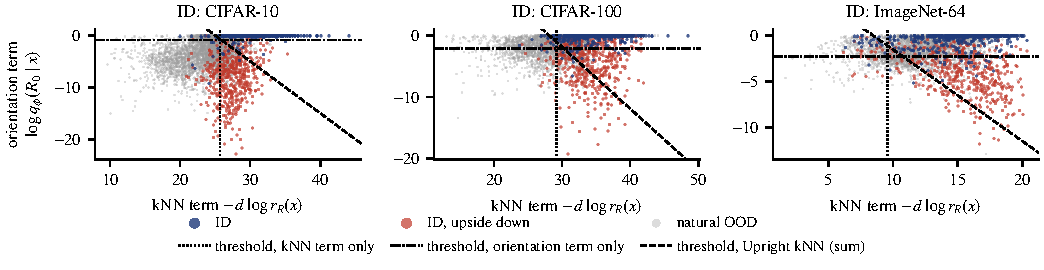
\includegraphics[width=\textwidth]{figs/fig_terms.pdf}
\caption{The two terms of Upright kNN on the final evaluation images (noise seed 0) for the three ID datasets with the lowest AUROC. Dotted: threshold of the kNN term alone that keeps 95\% of the ID images; dashed: the same for their sum (slope $-1$); images below and left of a line are declared OOD. Upside-down ID images (red) overlap the ID images (navy) in the kNN term but fall below the dashed line through the orientation term, whereas natural OOD images (grey) are separated mainly by the kNN term.}
\label{fig:terms}
\end{figure*}

\subsection{Six ID Datasets}
\label{sec:six}
Table~\ref{tab:main} gives the final evaluation. Upright kNN averages \oursMean\% AUROC over the six ID datasets, \priorGap{} points above the best prior method (CFS with a kNN head, \bestPriorMean\%); the rotation classifier reaches \rotMean\% and the best likelihood or statistic-based detector \bestEightMean\% (\bestEightName). The kNN rule on our features is a strong baseline in its own right (\ctMean\% basic, \tunedMean\% tuned), and Upright kNN improves on the tuned version most where orientation matters, CIFAR-10 (\oursCten{} vs \tunedCten\%) and ImageNet-64 (\oursIN{} vs \tunedIN\%). Against each prior method it wins \priorWinMin--\priorWinMax{} of the \nPairs{} pairs and loses at most \priorLossMax; against the tuned kNN it scores \wtlTuned. It loses to no comparison method on \nNoLoss{} pairs. The \nLost{} lost pairs are four upside-down sets (all to the rotation classifier), two pairs won by likelihood-based detectors (SVHN vs CelebA; ImageNet-64 vs iNaturalist, \pInInatNLL\% NLL vs \pInInat\% ours) and one pair won by the tuned kNN (CIFAR-100 vs CIFAR-10). The mean FPR95 is \FPRours\% for Upright kNN, \FPRbest\% for the tuned kNN and \FPRbestPrior\% for the best prior method (\FPRbestPriorName).

On upside-down ID images (Figure~\ref{fig:terms}), Upright kNN averages \vfOursAvg\% against \vfTunedAvg\% for the tuned kNN and \vfCfsKnnAvg\% for CFS (kNN head), e.g.\ \vfIN\% vs \vfINT\% on ImageNet-64. The rotation classifier is higher (\vfRotAvg\%), and so is the orientation term alone (\vfPoseAvg\%): in the sum, the kNN term varies from image to image while staying almost unchanged under flipping, which dilutes the drop of the orientation term. Upright kNN takes \cpuOurs\,s per image on a CPU, about 1/\cpuRatioNll{} of the likelihood (\cpuNll\,s) and 1/\cpuRatioDiffPath{} of DiffPath (\cpuDiffPath\,s).

\subsection{ImageNet-1K (OpenOOD v1.5)}
\label{sec:imagenet}
\begin{table}[t]\centering\footnotesize\setlength{\tabcolsep}{2.6pt}\renewcommand{\arraystretch}{0.92}
\begin{tabular}{@{}lcc|ccc|cc@{}}\toprule
 & \multicolumn{2}{c|}{OOD} & \multicolumn{3}{c|}{csID} & \multicolumn{2}{c}{Full spectrum}\\
Method & Near & Far & V2 & C & R & Near & Far\\\midrule
\inputrows{tab_imagenet.tex}
\bottomrule
\end{tabular}
\caption{OpenOOD v1.5 ImageNet-1K at 64$\times$64 with EDM2-XS (AUROC, \%; 1{,}000 images per set; frozen ImageNet-64 detectors). Near: SSB-hard, NINCO; far: iNaturalist, Textures, OpenImage-O; csID: ImageNet-V2, -C, -R against ImageNet val (ID); full spectrum: ID and csID images together as the positive class, weighted by the benchmark's set sizes. Marks as in Table~\ref{tab:main}; the csID columns are not marked.}
\label{tab:imagenet}
\end{table}
To test the method at scale we apply the frozen ImageNet-64 detectors, without any refitting, to the OpenOOD v1.5 ImageNet-1K benchmark~\cite{zhang2023openood}: ID is ImageNet validation~\cite{russakovsky2015imagenet}; near-OOD is SSB-hard~\cite{vaze2022openset} and NINCO~\cite{bitterwolf2023ninco}; far-OOD is iNaturalist~\cite{huang2021mos}, Textures~\cite{cimpoi2014dtd} and OpenImage-O~\cite{wang2022vim}; and the covariate-shifted ID sets (csID) are ImageNet-V2~\cite{recht2019imagenetv2}, ImageNet-C~\cite{hendrycks2019imagenetc} and ImageNet-R~\cite{hendrycks2021imagenetr}. Images used earlier for development or selection are excluded, leaving \inNFull{} ID images; Table~\ref{tab:imagenet} uses a fixed subsample of 1{,}000 images per set on which every method was run (on the full sets, Upright kNN gives \inNearFull\% near and \inFarFull\% far).

At 64$\times$64, Upright kNN reaches \inNear\% near-OOD and \inFar\% far-OOD AUROC, against \inNearPrior\% and \inFarPrior\% for the best prior method (CFS). It wins at least \inPriorWinMin{} of the five OOD sets against every prior method and loses only on iNaturalist, to NLL and TT (\inInatNLL\% and \inInatTT\% vs \inInat\%). Both terms contribute: the kNN term alone gives \inNearKnnT/\inFarKnnT\% and the orientation term alone \inNearPose/\inFarPose\%.

The csID columns show what a density-based detector does under covariate shift. ImageNet-V2 is treated as ID (\inVtwo\%), whereas corrupted and rendered images are flagged (ImageNet-C \inC\%, rising with severity from \inCsevOne\% to \inCsevFive\%; ImageNet-R \inR\%). The full-spectrum protocol~\cite{yang2023fsood} counts these as errors, so there Upright kNN (\inFSnear/\inFSfar\%) trails NLL (\inFSnearNLL/\inFSfarNLL\%), which ranks corrupted and rendered images as \emph{more} likely than clean ones (\inCNLL\% and \inRNLL\%). Whether covariate shift should be flagged depends on the application; Upright kNN flags it.

\begin{table}[t]\centering\footnotesize\setlength{\tabcolsep}{2.6pt}\renewcommand{\arraystretch}{0.92}
\begin{tabular}{@{}lc|cccc|cc@{}}\toprule
 & Near & \multicolumn{4}{c|}{Far} & & W/T/L\\
Method & NINCO & iNat & Tex & OI-O & Mean & Flip & of ours\\\midrule
\inputrows{tab_in256.tex}
\bottomrule
\end{tabular}
\caption{ImageNet at 256$\times$256 with ADM (AUROC, \%; \hNcom{} common images per set; the ImageNet-64 configuration unchanged; \hSeeds{} noise seeds for our rows and CFS). Flip: upside-down ID images. SSB-hard and ImageNet-C are left out because their 224-pixel images would be upsampled (see text). W/T/L over the four OOD sets; marks as in Table~\ref{tab:main}.}
\label{tab:in256}
\end{table}
\textbf{256$\times$256 with a different diffusion model.} We repeat the benchmark with the unconditional ADM model for 256$\times$256 ImageNet~\cite{dhariwal2021adm}, keeping every choice of the ImageNet-64 configuration ($R=1000$, the three blocks, $\sigma_1$, the head and its training) and a bank of 10 training images per class; all rows are evaluated on the \hNcom{} images per set for which the stored MSMA$^{*}$, DiffPath and GEPC statistics exist (Table~\ref{tab:in256}). SSB-hard and ImageNet-C are distributed at 224 pixels on the short side and must be upsampled, unlike ImageNet validation (median 375 pixels) and the other sets. Every feature-based detector then separates SSB-hard almost perfectly (\hSSB\% for ours, \hSSBCfs\% for CFS), a resolution shortcut rather than semantic novelty, so we leave both sets out at this resolution.\footnote{At 256$\times$256, the 32-image probe that CFS uses to rank its candidate blocks is passed through the network in chunks of four to fit GPU memory; everything else follows the official code.} Upright kNN is best on NINCO (\hNINCO\% vs \hNINCOPrior\% for the best prior method) and on upside-down images (\hVf\%, while every other method stays at chance, at most \hVfOtherMax\%), and second on far-OOD (\hFar\% vs \hFarPrior\% for CFS, a tie under the bootstrap). Its weak spot is OpenImage-O (\hOIO\% vs \hOIOCfs\% for CFS), where the kNN term itself fails. At this resolution the kNN term carries most of the near-OOD signal (\hNINCOKnnT\% on NINCO alone) and the orientation term the flip signal (\hVfPose\%).

\subsection{Is It Just kNN Plus a Rotation Classifier?}
\label{sec:fusion}
\begin{table}[t]\centering\footnotesize\setlength{\tabcolsep}{3pt}\renewcommand{\arraystretch}{0.92}
\begin{tabular}{@{}lccc@{}}\toprule
Score & Mean & Flip & W/T/L of ours\\\midrule
\inputrows{tab_fusion.tex}
\bottomrule
\end{tabular}
\caption{Principled sum vs.\ naive fusions (final evaluation, AUROC, \%; Mean and Flip as in Table~\ref{tab:main}). $z$-sum: sum of $z$-scores; Fisher: sum of log empirical ID $p$-values~\protect\cite{fisher1925}; both normalise each score with additional ID images (the development split), which Upright kNN does not need. W/T/L over the \nNatPairs{} natural-OOD pairs. This comparison was added after the frozen evaluation and reuses its images.}
\label{tab:fusion}
\end{table}
Upright kNN combines a nearest-neighbour score with a rotation predictor, so a natural question is whether any such combination works as well. Table~\ref{tab:fusion} compares the sum of Eq.~(\ref{eq:score}) with fusions that standardise the two scores using additional ID images. Fusing the kNN term with the image-space rotation classifier gives \fuRZ\% ($z$-sum) and \fuRF\% (Fisher), \emph{below} the kNN term alone; Upright kNN beats the $z$-sum fusion on \fuRZwtl{} (W/T/L) of the natural-OOD pairs. The classifier's confidence is high on upside-down images (\vfRotAvg\%) but poorly aligned with semantic novelty, so it adds noise to the kNN term on natural OOD sets. Fusing our own two terms is much closer (\fuOZ\%), but it needs extra ID images for normalisation, still loses more pairs than it wins against the principled sum (\fuOZwtl), and trades natural-OOD accuracy for flip detection. The exchange rate matters: setting $d=1$ in Eq.~(\ref{eq:score}) gives \fuDO\% (\fuDOwtl). On the development images, further variants are also worse on average: no temperature (\abNatD\%), estimating $\bar p$ directly with a rotated bank (\abNatF\%; \abCtenOrbit\% vs \abCtenOurs\% on CIFAR-10), training the head with rotated noise (\abNatG\%), or averaging the orientation term over four rotated test views (\abNatH\%), against \abNatA\% for Upright kNN; none of them raises the selection-data mean either.

\section{Analysis}
\label{sec:analysis}
\textbf{Why upside-down images are caught.} A vertical flip $\Vf$ equals a horizontal flip $\Hf$ composed with a half turn, $\Vf=\Hf\Rot{180}$. Natural ID data are close to left--right symmetric, which gives the following.
\begin{proposition}
\label{prop:mirror}
If $p(\Hf\mathbf{x})=p(\mathbf{x})$ for all $\mathbf{x}$, then $\bar p(\Vf\mathbf{x})=\bar p(\mathbf{x})$ and $\log p(\Vf\mathbf{x})-\log p(\mathbf{x})=\log P(\up\mid\Vf\mathbf{x})-\log P(\up\mid\mathbf{x})$.
\end{proposition}
\begin{proof}
For $\mathbf{G}\in\mG$ we have $\mathbf{G}\Hf=\Hf\mathbf{G}^{-1}$. Hence $\bar p(\Vf\mathbf{x})=\frac{1}{4}\sum_{\mathbf{G}}p(\Hf\mathbf{G}^{-1}\Rot{180}\mathbf{x})=\frac{1}{4}\sum_{\mathbf{G}}p(\mathbf{G}^{-1}\Rot{180}\mathbf{x})=\bar p(\mathbf{x})$, because $\mathbf{G}^{-1}\Rot{180}$ runs over $\mG$ once as $\mathbf{G}$ does. The second claim follows by subtracting Eq.~(\ref{eq:decomp}) at $\mathbf{x}$ from the same equation at $\Vf\mathbf{x}$.
\end{proof}
A flip therefore changes only the orientation term; a good content term is blind to it. This is what Figure~\ref{fig:method}(b) shows for one image (the flipped bird keeps its nearest neighbours, while the posterior moves to $180^\circ$) and Figure~\ref{fig:terms} for all of them: flipped ID images stay in the ID range of the kNN term and are pushed out by the orientation term. The proposition also explains the failure on SVHN (flip AUROC \vfSVHN\%; \vfSVHNPose\% for the orientation term alone): many digits (0, 1, 3, 8) look the same upside down.

\textbf{A mirror test for orientation information.} Proposition~\ref{prop:mirror} suggests a label-free probe. For any score $e$ and ID development images $\mathbf{x}_1,\dots,\mathbf{x}_n$, let $M(e)$ be the AUROC between $\{e(\mathbf{x}_i)\}$ and $\{e(\Vf\mathbf{x}_i)\}$. An ideal content term has $M=50\%$; $M$ near 100\% means that $e$ prefers upright images. For the kNN term computed from single blocks ($R=1$), $M$ grows with depth (CIFAR-10: 52.1\%, 67.3\% and 87.8\% at full, half and quarter resolution), while the same test with a horizontal flip stays at 49--56\% on the natural-image ID datasets. The kNN term of Upright kNN therefore still carries some orientation information (on CIFAR-10, $M=77.7\%$), which the orientation term complements. Across all blocks, $M$ is rank-correlated with the block's natural-OOD AUROC ($\rho=0.68$--$0.91$ on five ID datasets; $-0.53$ on SVHN, whose OOD sets differ mainly in colour and texture), so ID images alone indicate which blocks are useful for OOD detection.

\textbf{Data without a canonical orientation.} To see what happens when the ID data have no meaningful \emph{up}, we ran Upright kNN on EuroSAT aerial tiles~\cite{helber2019eurosat} with a diffusion U-Net trained on them, ten natural OOD sets and $R=5$ fixed in advance (a few duplicate tiles, whose neighbours all coincide, are skipped when estimating $d$). We expected the head to fall to chance; instead it predicts the rotation of held-out tiles with \eAcc\% accuracy (chance: 25\%), presumably from illumination and north-up acquisition. The orientation term therefore flags rotated tiles (\eRot\% AUROC for $90^\circ$ rotations, against \eRotKnnT\% for the kNN term), while natural-OOD detection is unchanged (\eOurs\% for Upright kNN and \eKnnT\% for its kNN term). Upright kNN thus estimates whatever orientation statistics the ID data have; when rotated inputs must count as ID, the orientation term should be dropped.

\textbf{Where the orientation term hurts.} The orientation term also reflects how familiar the content is to the ID model, which usually helps (CIFAR-10 vs CIFAR-100: \poseCtenCh\% for the orientation term alone vs \contentCtenCh\% for the kNN term) but can hurt: with CIFAR-100 as ID, the head finds CIFAR-10 images \emph{more} upright than CIFAR-100 images (orientation-term AUROC \poseChCten\%), which causes the single loss to the tuned kNN (\pChCten{} vs \pChCtenT\%).

\section{Limitations and Conclusion}
\label{sec:concl}
The orientation term encodes whatever orientation statistics the ID data have: it adds little when the content looks alike upside down (SVHN digits), and on aerial tiles it flags rotated inputs, which is unwanted when rotations should count as ID. Near-OOD remains hard: on ImageNet-64 the near-OOD AUROC stays around 70\%, and on the development images even the best of 2{,}738 scores we computed, selected per pair after the fact, stays below 80\% on CIFAR-100 vs CIFAR-10 and on SSB-hard and NINCO. The detector flags covariate shift, which full-spectrum OOD detection penalises, and at high resolution benchmark sets stored at a lower resolution than the ID images give every feature-based detector a shortcut that comparisons must control for. Finally, the bank features must be stored and searched, at a cost linear in the bank size.

Within these limits, a simple observation goes a long way: the log-density splits exactly into a rotation-invariant content term and an orientation term, and the single-pass features of a diffusion denoiser estimate the first well and, with a small head, the second as well. Restoring the missing factor turns a strong kNN baseline into a detector that beats \nPrior{} prior methods on six ID datasets under a frozen protocol and carries over to ImageNet at 64$\times$64 and, with another diffusion model, at 256$\times$256, at the cost of one network evaluation per image.

\bibliographystyle{named}
\bibliography{refs}

\end{document}
